\chapter{Documento de Diseño del Juego (GDD)}
\section{Características}
\begin{itemize}
	\item \textbf{Título:} N/A. \LaTeX \LaTeX \LaTeX \LaTeX
	\item \textbf{Plataforma:} \ac{PC} (Windows y Linux).
	\item \textbf{Género:} \acf{RTS}.
	\item \textbf{Idioma:} Inglés.
	\item \textbf{Clasificación:} PEGI 7\footnote{Web de la asociación https://pegi.info}
\end{itemize}

\section{Mecánicas}
La finalidad del juego es la de completar los distintos niveles de forma satisfactoria,
esto sucederá cuando eliminemos a todas las unidades enemigas desplegadas a lo largo del
nivel. Como herramienta para alcanzar este objetivo dispondremos de un ejercito a nuestro
mando el cual deberemos gestionar de forma efectiva para sortear los obstáculos y
desafios propuestos.

El jugador podrá seleccionar con el ratón las unidades exactas sobre las que quiere
lanzar la acción, seleccionar todas la unidades a su disposición mediante
atajos de teclado y/o deseleccionar en cualquier momento. Las acciones disponibles para
su uso serán las de desplazar las unidades, hacer que se queden a la espera y realizar
un ataque sobre las unidades rivales que se indiquen. Como puede verse en la 
imágen~\ref{fig:unit-selec}

El jugador perderá cuando todas sus unidades mueran.

\begin{figure}[ht]
\centering
\begin{minipage}[c]{0.45\linewidth}
	\hspace{1cm}
	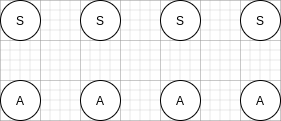
\includegraphics[width=0.7\textwidth]{imagenes/non-selection.png}
\end{minipage}
\begin{minipage}[c]{0.45\linewidth}
	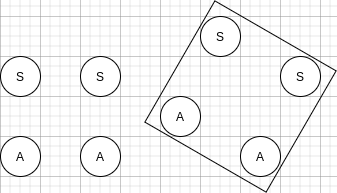
\includegraphics[width=0.7\textwidth]{imagenes/selection.png}
\end{minipage}	
\caption{MockUp selección.}
\label{fig:unit-selec}
\end{figure}

\section{Unidades}
Entre las unidades podemos encontrar diferentes arquetipos con carácteristicas propias
que nos permitiran crear variedad en las posibles soluciones a la hora de superar el
nivel.

Los distintos tipos son los siguientes:
\begin{itemize}
	\item \textbf{Soldado:} es la unidad más básica que podemos encontrar en el campo de
							guerra, esta armado con una espada y posee estadisticas
							bajas.
	\item \textbf{Arquero:} van equipado con arco y flechas para atacar a distancia a
							sus rivales, tiene menos resistencia que los soldados por
							lo que tendremos que protegerlos para asegurar su
							supervivencia.  
\end{itemize}

\section{Pantallas}
Al ejecutar el programa la primera pantalla que aparecerá será la de 
inicio~\ref{mockup_ini}. Se compone del título del juego, la fecha de lanzamiento,
el nombre del desarrollador y un mensaje que nos indica que tenemos que pulsar al tecla
\textit{entre} para continuar, esta pantalla se mantendrá hasta que el jugador presione
dicha tecla.

\begin{figure}[ht]
\centering
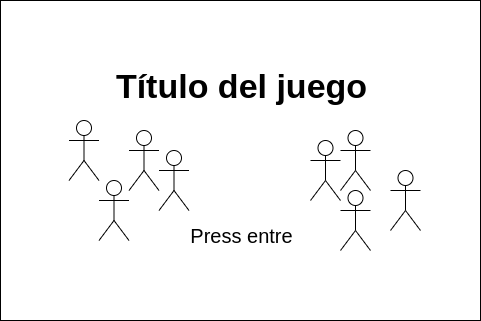
\includegraphics[width=0.45\textwidth]{imagenes/Pantalla_ini.png}
\caption{MockUp pantalla de inicio.}
\label{mockup_ini}
\end{figure}

Una vez pulsado el botón indicado se procederá a cargar el juego mientras se muestra
una barra que indica el progreso de cargado~\ref{mockup_carga}.

\begin{figure}[ht]
\centering
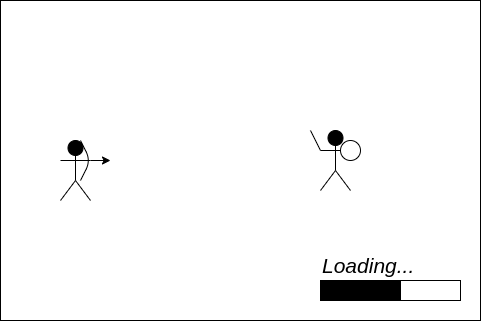
\includegraphics[width=0.45\textwidth]{imagenes/Pantalla_carga.png}
\caption{MockUp pantalla de carga.}
\label{mockup_carga}
\end{figure}

A continuación de la carga pasaremos directamente al escenario donde se desarrollará el
\textit{gameplay} y nos mantendremos en esta pantalla hasta que termine el juego, ya sea
por victoria o derrota del jugador~\ref{mockup_juego}.

\begin{figure}[ht]
\centering
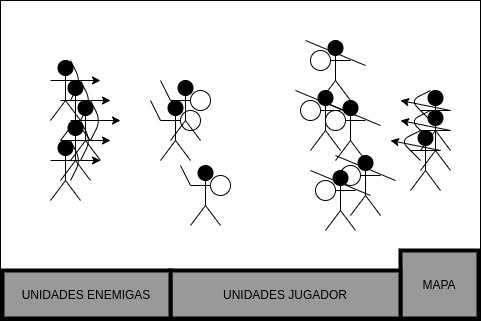
\includegraphics[width=0.45\textwidth]{imagenes/Pantalla_gameplay.png}
\caption{MockUp escenario juego.}
\label{mockup_juego}
\end{figure}

El final de la partida nos trae dos posibles escenarios, la victoria y la derrota. 
Para cada uno saldrá su respectivo mensaje~\ref{mockup_victoria}~\ref{mockup_derrota}
y pasado un momento se nos mandará automáticamente a la pantalla de
inicio~\ref{mockup_ini}.

\begin{figure}[ht]
\centering
\begin{minipage}[c]{0.45\linewidth}
	\hspace{9mm}
	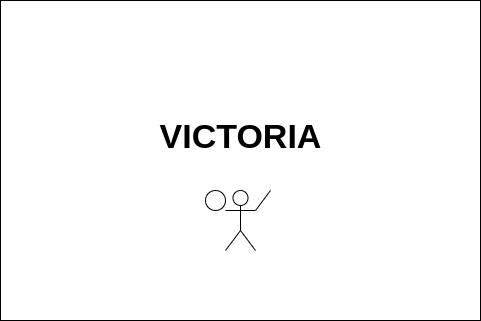
\includegraphics[width=0.7\textwidth]{imagenes/Pantalla_victoria.png}
	\caption{MockUp victoria.}
	\label{mockup_victoria}
\end{minipage}
\begin{minipage}[c]{0.45\linewidth}
	\hspace{9mm}
	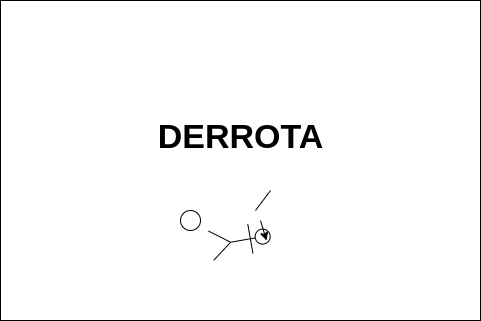
\includegraphics[width=0.7\textwidth]{imagenes/Pantalla_derrota.png}
	\caption{MockUp derrota.}
	\label{mockup_derrota}
\end{minipage}	
\end{figure}

Como última pantalla con la que el jugador podrá interactuar es la del menú de
pausa~\ref{mockup_pausa} en el cual se le dará la opción de salir o de volver a la
partida, mientras esta pantalla este activa la acción en el juego se paralizará hasta
que el jugador decida. 

\begin{figure}[ht]
\centering
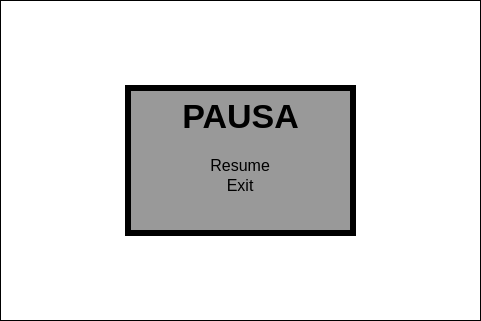
\includegraphics[width=0.45\textwidth]{imagenes/Pantalla_pausa.png}
\caption{MockUp menú de pausa.}
\label{mockup_pausa}
\end{figure}

\section{Estados del juego}

Una vez mostradas todas las posibles pantallas con las que podrá interactuar el jugador
es interesante dibujar un diagrama de flujo que plame sus conexiones y posibilidades
con el fin de crear una representación gráfica que sirva como esquema global.

Dicho esquema podemos encontrarlo en la figura~\ref{esq:flow_juego}.
\begin{figure}[ht]
\centering
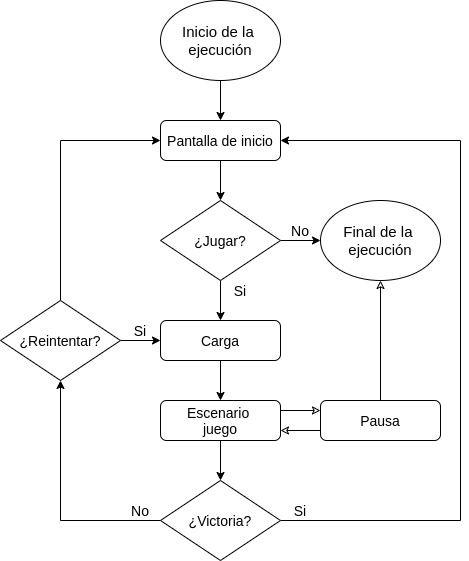
\includegraphics[width=0.45\textwidth]{imagenes/flow_ejecucion.png}
\caption{MockUp escenario juego.}
\label{esq:flow_juego}
\end{figure}